\begin{frame}
\frametitle{Xanadu}
\begin{itemize}
	\item Zwar verteiltet System aber dennoch Interessant
	\item 1960
	\item Langzeitprojekt (Open source in 1999)
	\item Ted Nelson
	\item "docuverse" - ein elektronische universale Bibliothek
	\item Mehr Framework als Programm
	\item Nie fertiggestellt, nur Prototypen und Modelle
\end{itemize}

\begin{figure}[htbp]
	\centering
	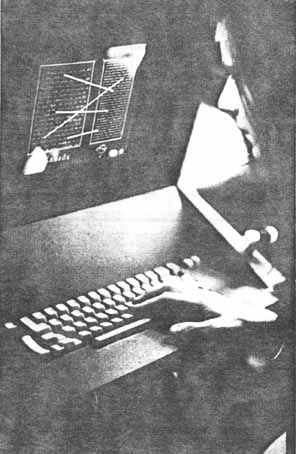
\includegraphics[width=0.22\textwidth]{images/xanadu}
\end{figure}

\end{frame}

\begin{frame}
\frametitle{Xanadu}
\framesubtitle{Funktionen}
\begin{itemize}
	\item Links / Strukturen
	\begin{itemize}
		\item Transklusions
		\item Jedes Dokument hat eine eindeutige Adresse
		\item Notizen, Kommentare
		\item Verknüpfungen innerhalb der Dokumente zu anderen Dokumenten
	\end{itemize}
\end{itemize}
\end{frame}
